
\chapter{Language Design and Type System}
In this chapter, we'll design a subset of R with types and see how types and their operations could map to WASM generation.
\section{Design Goals}
Some reader at this point might be wondering why subset of R and why with types, why not just compile R to WASM. 
R is notoriously hard to compile to statically typed byte-code. The first reason is typing. 
\newline

\noindent Let's take the following code.
\begin{lstlisting}
  x <- some_function()
\end{lstlisting}
WASM on the other hand is expecting variable \texttt{x} to have a type. There's 
\texttt{any} type in WASM. Maybe we can try mapping it to \texttt{anyref}. A reference to \texttt{any} element by the WASM GC proposal.
So now we have
\begin{lstlisting}
  (local $x anyref) // A tagged union can be also used.
\end{lstlisting}
Then, let's have a binary operation \texttt{x + y}, where \texttt{y} is also \texttt{anyref}.
Now we need to implement a generic function for plus operator that can potentially dispatch to all types of that function.
\begin{lstlisting}
  if x is int && y is int:
    add_int(x, y)
  if x is double && y is double:
    add_double(x, y)
  ...
\end{lstlisting}
This code will continue for every type and its combination. We'd have to also include promotion logic 
inside this code. Then x is int needs \texttt{try\_cast} as well. 
We'll need to do such generic function for every operation and functions. Some will be 
impossible to cover. This is essentially re-implementing the R interpreter.
Thus we fixate on R that's well-typed and the type is known or inferrable at compile time.

Moreover, we will see the same issue of dynamic dispatching when R variables change types.
\begin{lstlisting}
  x <- 5        # numeric
  x <- "hello"  # now a string
  x <- list()   # now a list
\end{lstlisting}
This bounds us to either writing generic functions or using wrappers like a tagged union, which will 
limit our performance and waste memory.

Moreover, R uses lazy evaluation for function arguments; they're only evaluated when actually used:
\begin{lstlisting}
  f <- function(x, y) { if (x > 0) y else 0 }
  f(5, expensive_computation())  # expensive_computation() never runs!
\end{lstlisting}
This requires complex bookkeeping that's hard to optimize. Then, we have 
one of the main challenging feature with any attempts of ahead-of-compilation.
The reflection. R code can inspect and modify itself at runtime:
\begin{lstlisting}
  x <- quote(a + b)  # capture unevaluated expression
  eval(x)            # evaluate it later
\end{lstlisting}

\noindent Lastly, many R functions evaluate arguments in non-standard ways:
\begin{lstlisting}
  subset(df, age > 30)  # 'age' isn't a variable, it's a column name!
\end{lstlisting}
This is extremely difficult to analyze statically.

In conclusion, all those issues outlined above, is not impossible to compile. However, they require
complex implementation and huge performance and memory trade-offs. For these, reasons it's important
for me to define the subset of R, which I can compile and limit the scope without losing R's main functionalities and purposes.

\section{Typed R-like Language}
This section presents the design of a statically-typed programming language inspired by R's syntax, which we refer to as the \textit{Typed R-like Language}. The language maintains R's characteristic features such as the left-assignment operator (\texttt{<-}), first-class functions, and vector-oriented programming, while introducing a static type system to enable ahead-of-time compilation to WebAssembly.

Table \ref{tab:r-typed-r-comparison0} compares the data types supported by R and Typed R, showing which primitive and composite types are available in each language.

\begin{table}[h]
\centering
\begin{tabular}{|l|c|c|}
\hline
\textbf{Language Feature (Types)} & \textbf{R} & \textbf{Typed R} \\
% Basic Data Types
\hline
Integers & \checkmark & \checkmark \\
Doubles & \checkmark & \checkmark \\
Booleans & \checkmark & \checkmark \\
Strings & \checkmark & $\times$ \\
NULL/NA values & \checkmark & $\times$ \\
\hline

% Composite Data Types
Vectors & \checkmark & \checkmark \\
Matrices & \checkmark & $\times$ \\
Lists & \checkmark & $\times$ \\
Data frames & \checkmark & $\times$ \\
Arrays & \checkmark & $\times$ \\
\hline
\end{tabular}
\caption{Comparison of language features supported by R and Typed R}
\label{tab:r-typed-r-comparison0}
\end{table}

Table \ref{tab:r-typed-r-comparison1} presents a broader comparison of language features, including type system properties, functional programming capabilities, and advanced features that distinguish Typed R from standard R.

\begin{table}[h]
\centering
\begin{tabular}{|l|c|c|}
\hline
\textbf{Language Feature} & \textbf{R} & \textbf{Typed R} \\
% Basic Data Types
\hline

Static typing & $\times$ & \checkmark \\
First-class functions & \checkmark & \checkmark \\
Vector operations & \checkmark & \checkmark \\
Math operations & \checkmark & \checkmark \\
Control flow & \checkmark & \checkmark \\
Higher-order functions & \checkmark & \checkmark \\
Lexical scoping & \checkmark & \checkmark \\
Named arguments & \checkmark & \checkmark \\
Variable arguments (...) & \checkmark & \checkmark \\
\hline
Reflection & \checkmark & $\times$ \\
Runtime type changes & \checkmark & $\times$ \\
Non-standard evaluation (NSE) & \checkmark & $\times$ \\
Lazy evaluation & \checkmark & $\times$ \\
Copy-on-modify semantics & \checkmark & $\times$ \\
Garbage collection & \checkmark & \checkmark \\
Operator overloading & \checkmark & $\times$  \\
Attributes/metadata & \checkmark & $\times$  \\
Method dispatch (S3/S4/R6) & \checkmark & $\times$  \\

\hline
\end{tabular}
\caption{Comparison of language types supported by R and Typed R}
\label{tab:r-typed-r-comparison1}
\end{table}

The design philosophy emphasizes a familiar R-like syntax while ensuring type safety and efficient compilation to WebAssembly. Unlike dynamically-typed R,
all type information is resolved at compile time, enabling optimized code generation and early error detection. It's also worth to mention that
implementation of those features take a lot of engineering time and effort. Therefore, I have only implemented
what I see as essential and most used for demonstrating the point of this thesis.
\clearpage
\section{Syntax}

\subsection{Overview}
The syntax of the Typed R-like Language closely follows R conventions with extensions for explicit type annotations. The language retains R's characteristic left-assignment operator (\texttt{<-}), first-class functions, and vector-oriented syntax. Type annotations are introduced where needed for static typing, using a colon notation (e.g., \texttt{x: int}). This section presents the abstract grammar, lexical elements, and illustrative examples of core syntactic constructs.

\subsection{Abstract Grammar}

The abstract grammar uses the following notation: $e$ denotes expressions (computations that produce values), $s$ denotes statements (computations that perform actions and may bind variables), and $p$ denotes function parameters. Binary operations are represented by $\oplus$ (arithmetic: \texttt{+}, \texttt{-}, \texttt{*}, \texttt{/}, \texttt{\%\%}; comparison: \texttt{==}, \texttt{!=}, \texttt{<}, \texttt{<=}, \texttt{>}, \texttt{>=}; logical: \texttt{\&}, \texttt{|}), and unary operations by $\ominus$ (negation: \texttt{-}, logical not: \texttt{!}). Type annotations are denoted by $\tau$, variables by $x$, integer literals by $n$, and floating-point literals by $d$.

\begin{align*}
e ::= &\ x \quad \text{(variable)} \\
    &\mid n \mid d \mid \texttt{true} \mid \texttt{false} \quad \text{(literals)} \\
    &\mid \texttt{function}(p_1, \ldots, p_n): \tau\ \{\ e\ \} \quad \text{(function definition)} \\
    &\mid e_1(e_2, \ldots, e_n) \quad \text{(function call)} \\
    &\mid e_1(x_1{=}e_2, \ldots, x_n{=}e_n) \quad \text{(named argument call)} \\
    &\mid e_1 \oplus e_2 \quad \text{(binary operation)} \\
    &\mid \ominus e \quad \text{(unary operation)} \\
    &\mid \texttt{c}(e_1, \ldots, e_n) \quad \text{(vector construction)} \\
    &\mid e_1:e_2 \quad \text{(range sequence)} \\
    &\mid e_1[e_2] \quad \text{(vector indexing)} \\
    &\mid \texttt{if}\ e_1\ \{\ e_2\ \}\ \texttt{else}\ \{\ e_3\ \} \quad \text{(conditional)} \\
    &\mid \{\ e_1;\ \ldots;\ e_n\ \} \quad \text{(block)} \\
s ::= &\ x \gets e \quad \text{(assignment)} \\
    &\mid x: \tau \gets e \quad \text{(typed assignment)} \\
    &\mid x \ll\gets e \quad \text{(superassignment)} \\
    &\mid e \quad \text{(expression statement)} \\
    &\mid \texttt{return}(e) \quad \text{(return)} \\
    &\mid \texttt{for}\ (x\ \texttt{in}\ e)\ \{\ s\ \} \quad \text{(for loop)} \\
    &\mid \texttt{while}\ (e)\ \{\ s\ \} \quad \text{(while loop)} \\
p ::= &\ x: \tau \quad \text{(required parameter)} \\
    &\mid x: \tau = e \quad \text{(parameter with default)} \\
    &\mid \ldots \quad \text{(varargs)}
\end{align*}


\subsection{Lexical Elements}

The language uses the following lexical tokens:

\begin{itemize}
    \item \textbf{Keywords:} \texttt{function}, \texttt{if}, \texttt{else}, \texttt{for}, \texttt{in}, \texttt{while}, \texttt{return}
    \item \textbf{Type keywords:} \texttt{int}, \texttt{double}, \texttt{void}, \texttt{logical}, \texttt{vector}
    \item \textbf{Operators:}
    \begin{itemize}
        \item Assignment: \texttt{<-} (assignment), \texttt{<<-} (super-assignment)
        \item Arithmetic: \texttt{+}, \texttt{-}, \texttt{*}, \texttt{/}, \texttt{\%\%} (modulo)
        \item Comparison: \texttt{==}, \texttt{!=}, \texttt{<}, \texttt{<=}, \texttt{>}, \texttt{>=}
        \item Logical: \texttt{\&} (and), \texttt{|} (or), \texttt{!} (not)
        \item Range: \texttt{num1} \texttt{:} \texttt{num2} (sequence generation)
        \item Type annotation: \texttt{:} (in declaration context)
        \item Function arrow: \texttt{->} (in type signatures)
    \end{itemize}
    \item \textbf{Delimiters:} \texttt{(}, \texttt{)}, \texttt{\{}, \texttt{\}}, \texttt{[}, \texttt{]}, \texttt{,}
    \item \textbf{Literals:} Numeric literals, logical literals (\texttt{TRUE}, \texttt{FALSE})
    \item \textbf{Identifiers:} Alphanumeric sequences starting with a letter or underscore
    \item \textbf{Special:} \texttt{...} (varargs placeholder)
\end{itemize}

\subsection{Illustrative Examples}

This subsection demonstrates the syntax through concrete examples, organized by language construct.

\paragraph{Variable Assignment}

Variables are declared using the left-assignment operator with optional type annotations:

\begin{lstlisting}[language=R, caption={Variable assignment examples}]
# Simple assignment with type inference
x <- 10

# Assignment with explicit type annotation
y: int <- 20

# Vector assignment
vec <- c(1, 2, 3)
\end{lstlisting}

\paragraph{Super-assignment}

R distinguishes between assigning a variable in the current scope versus an outer scope with different syntax, unlike other popular dynamic languages like Python or Javascript. Typed R retains this distinction. 

\begin{lstlisting}[language=R, caption={Super-assignment example}, label={r_superassignment}]
outer <- function() {
    x <- 0
    inner <- function() {
        x <<- 10  # Modifies x in outer scope
    }
    inner()
    return(x)  # Returns 10
}
\end{lstlisting}
Note that in Code fragment~\ref{r_superassignment}, Typed R syntax is identical to R. For trivial cases like this, type inference can help significantly, as discussed in the type system section.

\paragraph{Functions}

Functions are first-class values defined using the \texttt{function} keyword:

\begin{lstlisting}[language=R, caption={Function definition examples in typed R}]
# Simple function with type annotations
add <- function(a: int, b: int): int {
    return(a + b)
}

# Function returning a vector
create_vector <- function(): vector<double> {
    return(c(1.0, 2.0, 3.0))
}

# Higher-order function
apply_twice <- function(f: int -> int, x: int): int {
    return(f(f(x)))
}

\end{lstlisting}
First-class values mean they are essentially the same as objects like vectors. They can be passed as parameters, saved to variables, and returned from functions.

\paragraph{Control Flow}

Conditional expressions use \texttt{if-else} syntax similar to R:

\begin{lstlisting}[language=R, caption={Conditional examples in typed R}]
# If statement
if (x > 0) {
    print(x)
}

# If-else statement
if (x > 0) {
    y <- 1
} else {
    y <- -1
}

# If expression (returns value)
result <- if (x > 0) { 1 } else { -1 }
\end{lstlisting}
Note that R's syntactic sugar for single-expression conditionals (\texttt{if (expr) 1 else 0} without brackets) is not implemented in our compiler.

\paragraph{Loops}

Two loop constructs are provided: \texttt{for} and \texttt{while}.

\begin{lstlisting}[language=R, caption={Loop examples}]
# For loop iterating over range
for (i in 1:10) {
    print(i)
}

# For loop iterating over vector
vec <- c(1, 2, 3, 4, 5)
for (x in vec) {
    print(x)
}

# While loop
i <- 1
sum <- 0
while (i <= 5) {
    sum <- sum + i
    i <- i + 1
}
\end{lstlisting}

\paragraph{Blocks and Closures}

Blocks consist of zero or more statements followed by an optional tail expression. The tail expression (final expression without semicolon) determines the block's value:

\begin{lstlisting}[language=R, caption={Block with tail expression}]
f <- function(x: int): int {
    y <- x * 2
    z <- y + 1
    z  # Tail expression - returned automatically
}
\end{lstlisting}

Only functions create new scopes; blocks, if-statements, and loops share their enclosing function's scope. A \textbf{closure} is a function that captures variables from its defining environment. When a function references a variable from an outer function scope, that variable remains accessible even after the outer function returns. Super-assignment (\texttt{<<-}) modifies captured variables by searching enclosing function scopes.

Example demonstrating closure:
\begin{lstlisting}[language=R, caption={Closure example}]
make_counter <- function(start: int): () -> int {
    count <- start
    function(): int {
        count <<- count + 1
        return(count)
    }
}

counter <- make_counter(0)
print(counter())  # Prints 1
print(counter())  # Prints 2
\end{lstlisting}

\section{Type System}
The type system ensures type safety through static analysis while supporting type inference to maintain concise syntax and ease of development. Type inference fails for programs lacking sufficient type information, requiring explicit annotations in those cases. The type grammar defines three major categories:

\begin{align*}
\tau ::= & \; num \mid \texttt{void} && \text{(base type)} \\
       | & \; \tau\texttt{[]} && \text{(vector type)} \\
       | & \; (\tau_1, \ldots, \tau_n) \to \tau && \text{(function type)} \\[0.5em]
num    ::= & \; \texttt{int} \mid \texttt{double} \mid \texttt{bool} && \text{(numeric types)}
\end{align*}

Typed R builds upon three core numeric types that align naturally with WebAssembly's type system. The \texttt{int} type represents 32-bit signed integers, mapping directly to WebAssembly's \texttt{i32} primitive, with values ranging from $-2^{31}$ to $2^{31}-1$. The \texttt{double} type provides 64-bit IEEE 754 floating-point numbers, corresponding to WebAssembly's \texttt{f64}, matching R's default numeric type for statistical computations. Boolean logic uses the \texttt{logical} type with R-style literals \texttt{TRUE} and \texttt{FALSE}, represented as \texttt{i32} in WebAssembly where zero means false and non-zero means true. Finally, \texttt{void} denotes the absence of a value for functions that perform side effects without returning data.

Beyond primitive types, vectors form the core composite structure. Vectors are homogeneous arrays parameterized by element type:

\begin{lstlisting}[language=R, caption={Vector type examples}]
# Vector of integers
v1: vector<int> <- c(1, 2, 3)

# Vector of doubles
v2: vector<double> <- c(1.5, 2.5, 3.5)

# Vector operations (component-wise)
v3: vector<double> <- v2 + c(1.0, 2.0, 3.0)
\end{lstlisting}

Vectors support component-wise arithmetic operations when both operands have compatible vector types.

Function types complete the type system by encoding callable values with their parameter and return types. The simplest form, \texttt{int -> int}, describes a function accepting a single integer and producing an integer result. Multi-parameter functions extend this: \texttt{int, int -> double} takes two integers and returns a double. Higher-order functions naturally fit this notation, such as \texttt{(int -> int) -> int}, which accepts a function mapping integers to integers and returns an integer. Complex signatures like \texttt{int, (int, int -> int) -> int} combine these patterns, taking both a plain integer and a binary function as parameters. To avoid ambiguity in expressions like \texttt{int -> int -> int}, we require explicit parentheses in type annotations, ensuring each signature has exactly one interpretation.

Type promotion follows a subtyping hierarchy shown in Figure~\ref{fig:subtyping-hierarchy}. Logical values can be used wherever integers are expected, and integers can be used wherever doubles are expected, creating the chain \texttt{logical $<:$ int $<:$ double}. Vectors are covariant with respect to their element types, meaning \texttt{vector<int>} can be used where \texttt{vector<double>} is expected, preserving the subtyping relationship across composite types.
\begin{figure}[htbp]
\centering
\makebox[\textwidth][c]{%
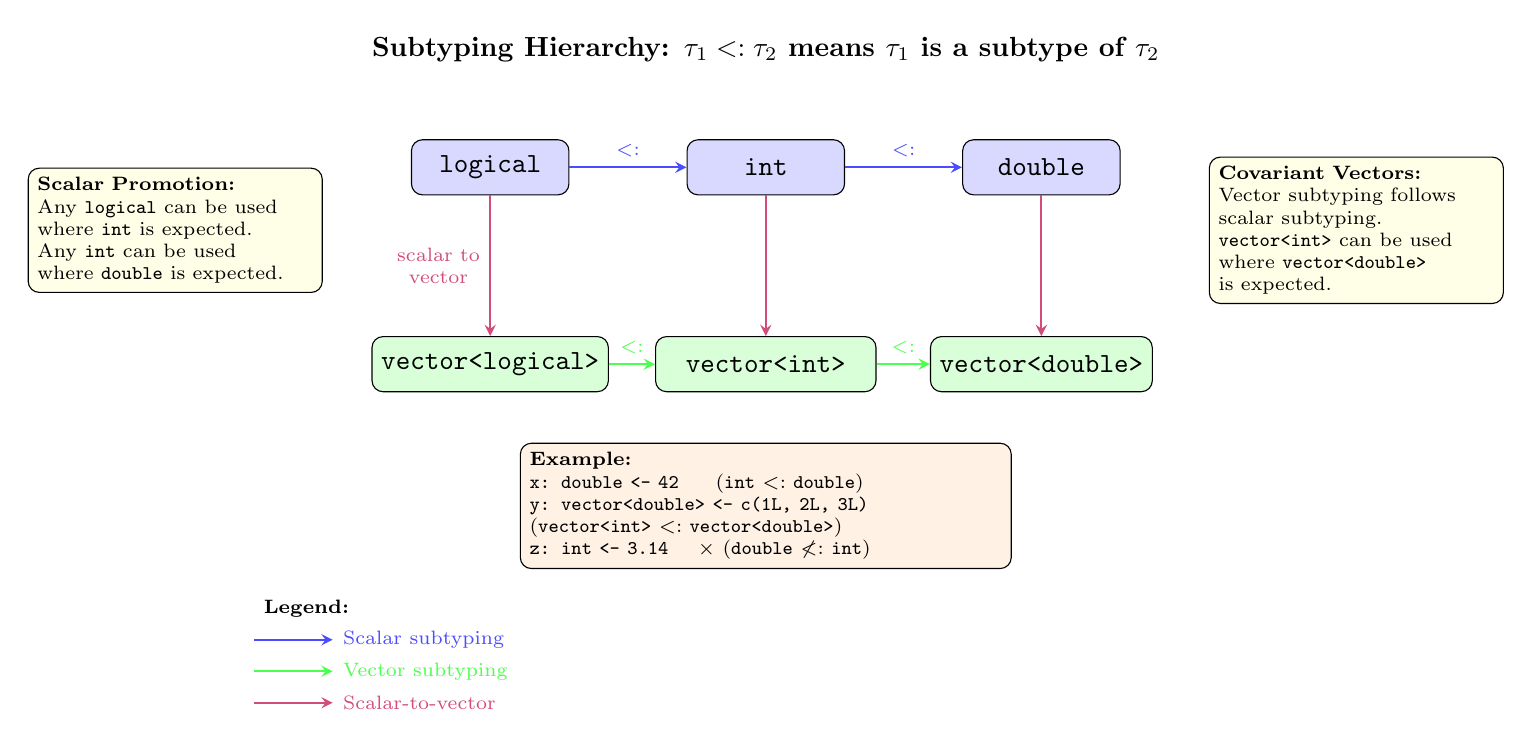
\begin{tikzpicture}[
    node distance=1.2cm,
    every node/.style={font=\small},
    scalarnode/.style={rectangle, draw, rounded corners, fill=blue!15, minimum width=2cm, minimum height=0.7cm, align=center, font=\ttfamily},
    vectornode/.style={rectangle, draw, rounded corners, fill=green!15, minimum width=2.8cm, minimum height=0.7cm, align=center, font=\ttfamily},
    subtype/.style={->, >=stealth, thick, blue!70},
    vecsubtype/.style={->, >=stealth, thick, green!70},
    crosssubtype/.style={->, >=stealth, thick, purple!70},
]

% Title
\node[font=\bfseries] at (0, 5.5) {Subtyping Hierarchy: $\tau_1 <: \tau_2$ means $\tau_1$ is a subtype of $\tau_2$};

% Scalar types (top row)
\node[scalarnode] (logical) at (-3.5, 4) {logical};
\node[scalarnode] (int) at (0, 4) {int};
\node[scalarnode] (double) at (3.5, 4) {double};

% Scalar subtyping arrows
\draw[subtype] (logical) -- node[above, font=\scriptsize] {$<:$} (int);
\draw[subtype] (int) -- node[above, font=\scriptsize] {$<:$} (double);

% Vector types (bottom row)
\node[vectornode] (veclogical) at (-3.5, 1.5) {vector<logical>};
\node[vectornode] (vecint) at (0, 1.5) {vector<int>};
\node[vectornode] (vecdouble) at (3.5, 1.5) {vector<double>};

% Vector subtyping arrows
\draw[vecsubtype] (veclogical) -- node[above, font=\scriptsize] {$<:$} (vecint);
\draw[vecsubtype] (vecint) -- node[above, font=\scriptsize] {$<:$} (vecdouble);

% Scalar to vector arrows (covariant)
\draw[crosssubtype] (logical) -- node[left, font=\scriptsize, align=center] {scalar to\\vector} (veclogical);
\draw[crosssubtype] (int) -- (vecint);
\draw[crosssubtype] (double) -- (vecdouble);

% Annotation boxes
\node[draw, rounded corners, fill=yellow!10, align=left, font=\scriptsize, text width=3.5cm] at (-7.5, 3.2) {
\textbf{Scalar Promotion:}\\
Any \texttt{logical} can be used\\
where \texttt{int} is expected.\\
Any \texttt{int} can be used\\
where \texttt{double} is expected.
};

\node[draw, rounded corners, fill=yellow!10, align=left, font=\scriptsize, text width=3.5cm] at (7.5, 3.2) {
\textbf{Covariant Vectors:}\\
Vector subtyping follows\\
scalar subtyping.\\
\texttt{vector<int>} can be used\\
where \texttt{vector<double>}\\
is expected.
};

% Example box
\node[draw, rounded corners, fill=orange!10, align=left, font=\scriptsize, text width=6cm] at (0, -0.3) {
\textbf{Example:}\\
\texttt{x: double <- 42} \quad $\checkmark$ (\texttt{int} $<:$ \texttt{double})\\
\texttt{y: vector<double> <- c(1L, 2L, 3L)} \quad $\checkmark$ (\texttt{vector<int>} $<:$ \texttt{vector<double>})\\
\texttt{z: int <- 3.14} \quad $\times$ (\texttt{double} $\not<:$ \texttt{int})
};

% Legend
\node[font=\scriptsize\bfseries, anchor=west] at (-6.5, -1.6) {Legend:};
\draw[subtype] (-6.5, -2) -- (-5.5, -2) node[anchor=west, font=\scriptsize] {Scalar subtyping};
\draw[vecsubtype] (-6.5, -2.4) -- (-5.5, -2.4) node[anchor=west, font=\scriptsize] {Vector subtyping};
\draw[crosssubtype] (-6.5, -2.8) -- (-5.5, -2.8) node[anchor=west, font=\scriptsize] {Scalar-to-vector};

\end{tikzpicture}%
}
\caption{Subtyping hierarchy showing scalar type promotion (\texttt{logical} $<:$ \texttt{int} $<:$ \texttt{double}) and covariant vector subtyping (\texttt{vector<logical>} $<:$ \texttt{vector<int>} $<:$ \texttt{vector<double>}). Scalar-to-vector conversions preserve the subtyping relationship, allowing implicit promotion in both scalar and vector contexts.}
\label{fig:subtyping-hierarchy}
\end{figure}

The language provides no user-creatable subtyping; we don't support R's S3 system or OOP features in Typed R.
\clearpage

Type checking follows a bidirectional approach\cite{bidirectional_typing} that combines bottom-up inference and top-down checking. Bottom-up inference derives expression types from literal values and operator signatures, while top-down checking uses function return types and variable annotations to provide expected types. Unification solves type constraints to determine concrete types, incorporating the subtyping rules to enable implicit type promotion.


\begin{figure}[htbp]
\centering
\begin{tikzpicture}[
    node distance=0.4cm,
    every node/.style={font=\small},
    astnode/.style={rectangle, draw, minimum width=2.2cm, minimum height=0.7cm, align=center, fill=gray!5},
    typenode/.style={ellipse, draw, fill=blue!15, minimum width=1.8cm, minimum height=0.6cm, align=center, font=\small\ttfamily},
    constraint/.style={rectangle, rounded corners, draw, fill=orange!15, minimum width=3cm, minimum height=0.6cm, align=center, font=\footnotesize},
    arrow/.style={->, >=stealth, thick},
    typearrow/.style={->, >=stealth, dashed, blue, thick},
    checkarrow/.style={->, >=stealth, red!70, thick}
]

% Title
\node[font=\bfseries] at (0, 4.2) {Type Checking: \texttt{a: double <- 3.5}};

% AST Nodes
\node[astnode] (assign) at (0, 3) {Assignment\\$\texttt{a} \leftarrow$};
\node[astnode] (decl) at (-3, 1.8) {Variable\\Declaration: \texttt{a}};
\node[astnode] (literal) at (3, 1.8) {Literal\\Expression: \texttt{3.5}};

% Type annotations
\node[typenode] (decltype) at (-3, 0.6) {double};
\node[typenode] (littype) at (3, 0.6) {double};

% Connections
\draw[arrow] (assign) -- (decl);
\draw[arrow] (assign) -- (literal);

% Type inference (bottom-up)
\draw[typearrow] (literal) -- node[right, font=\scriptsize, text=blue!70] {infer} (littype);

% Type annotation (top-down)
\draw[typearrow] (decl) -- node[left, font=\scriptsize, text=blue!70] {annotate} (decltype);

% Unification
\node[constraint] (unify) at (0, 0.6) {Unification Check};
\draw[checkarrow] (decltype) -- (unify);
\draw[checkarrow] (littype) -- (unify);

% Success indicator
\node[constraint, fill=green!20] (success) at (0, -0.4) { Type Check Passes: \texttt{double = double}};
\draw[arrow, green!70!black, thick] (unify) -- (success);

% Step-by-step annotation boxes
\node[anchor=west, font=\scriptsize, align=left, draw, rounded corners, fill=yellow!10, minimum width=4.5cm] at (5, 3) {
\textbf{Step 1: Top-down}\\
Parse annotation \texttt{a: double}\\
Expected type: \texttt{double}
};

\node[anchor=west, font=\scriptsize, align=left, draw, rounded corners, fill=yellow!10, minimum width=4.5cm] at (5, 1.5) {
\textbf{Step 2: Bottom-up}\\
Infer literal \texttt{3.5}\\
Inferred type: \texttt{double}
};

\node[anchor=west, font=\scriptsize, align=left, draw, rounded corners, fill=yellow!10, minimum width=4.5cm] at (5, 0) {
\textbf{Step 3: Unify}\\
Check: \texttt{double} $\stackrel{?}{=}$ \texttt{double}\\
Result: \textcolor{green!70!black}{\textbf{Success!}}
};

% Legend
\node[font=\scriptsize\bfseries, anchor=west] at (-5, -1.3) {Legend:};
\draw[arrow] (-5, -1.7) -- (-4.2, -1.7) node[anchor=west, font=\scriptsize] {AST structure};
\draw[typearrow] (-5, -2.1) -- (-4.2, -2.1) node[anchor=west, font=\scriptsize] {Type flow};
\draw[checkarrow] (-5, -2.5) -- (-4.2, -2.5) node[anchor=west, font=\scriptsize] {Unification};

\end{tikzpicture}
\caption{Bidirectional type checking for variable assignment. The type annotation \texttt{double} provides the expected type (top-down), while the literal \texttt{3.5} has its type inferred as \texttt{double} (bottom-up). The unification step verifies that both types match, allowing the assignment to proceed.}
\label{fig:type-checking-simple}
\end{figure}

The basic algorithm works as follows: when type-checking an expression, if the type can be inferred from the expression itself (bottom-up), that inferred type is used. If an explicit type annotation is provided (top-down), the annotation is used as the expected type. When both are present, unification checks that the inferred type is compatible with (a subtype of) the annotated type. If neither inference nor annotation provides type information, type checking fails.

Type annotations are required for function parameters, function return types (when not inferrable from return statements), and ambiguous variable declarations. For example, in \texttt{a: double <- 3.5}, the literal \texttt{3.5} infers as \texttt{double} (bottom-up), the annotation expects \texttt{double} (top-down), and unification confirms they match (see Figure~\ref{fig:type-checking-simple}). The expression \texttt{3 + 2.5} demonstrates type promotion: \texttt{3} infers as \texttt{int} but is promoted to \texttt{double} through subtyping to match \texttt{2.5}, evaluating as \texttt{3.0 + 2.5 = 5.5}.

We do not formalize the complete type inference algorithm here, as bidirectional type inference is well-studied in programming language literature\cite{bidirectional_typing}. Our implementation follows standard techniques, extended with the subtyping hierarchy described in Section~\ref{fig:subtyping-hierarchy}.

The formal type system uses inference rules with typing judgments of the form $\Gamma \vdash e : \tau$, read as "under typing context $\Gamma$, expression $e$ has type $\tau$." A typing context maps variable names to their types, defined as $\Gamma ::= \emptyset \mid \Gamma, x:\tau$, where $\emptyset$ is the empty context and $\Gamma, x:\tau$ extends context $\Gamma$ with a binding of variable $x$ to type $\tau$. We write $x:\tau \in \Gamma$ when $\Gamma$ contains the binding. Rules appear in natural deduction style with premises above the horizontal line and conclusions below; axioms have no premises. Our type system follows standard approaches from programming language theory~\cite{types_and_pl}, extended with subtyping for numeric promotion and vector operations.

Subtyping defines when one type can safely substitute for another. We write $\tau_1 <: \tau_2$ to mean "$\tau_1$ is a subtype of $\tau_2$" (equivalently, $\tau_1$ can be used wherever $\tau_2$ is expected). Every type is a subtype of itself, and the numeric promotion hierarchy establishes base cases:

\begin{mathpar}
\inferrule*[right=S-Refl]
    {\ }
    {\tau <: \tau}

\and

\inferrule*[right=S-LogicalInt]
    {\ }
    {\texttt{logical} <: \texttt{int}}

\and

\inferrule*[right=S-IntDouble]
    {\ }
    {\texttt{int} <: \texttt{double}}
\end{mathpar}

\textsc{S-Refl} states that any type is a subtype of itself (reflexivity). \textsc{S-LogicalInt} allows logical values to be used as integers. \textsc{S-IntDouble} allows integers to be promoted to doubles, enabling mixed arithmetic like \texttt{3 + 2.5}. Subtyping is transitive, allowing chains like $\texttt{logical} <: \texttt{int} <: \texttt{double}$:

\begin{mathpar}
\inferrule*[right=S-Trans]
    {\tau_1 <: \tau_2 \\ \tau_2 <: \tau_3}
    {\tau_1 <: \tau_3}
\end{mathpar}

If $\tau_1$ can be used as $\tau_2$, and $\tau_2$ can be used as $\tau_3$, then $\tau_1$ can be used as $\tau_3$, giving us $\texttt{logical} <: \texttt{double}$ automatically. Vectors are covariant in their element type:

\begin{mathpar}
\inferrule*[right=S-Vector]
    {\tau_1 <: \tau_2}
    {\texttt{vector}\langle\tau_1\rangle <: \texttt{vector}\langle\tau_2\rangle}
\end{mathpar}

When element type $\tau_1$ is a subtype of $\tau_2$, a vector of $\tau_1$ can be used where a vector of $\tau_2$ is expected. For example, \texttt{vector<int>} $<:$ \texttt{vector<double>}, so an integer vector can be passed to a function expecting a double vector. The subsumption rule connects subtyping to the type system, enabling implicit type promotion:

\begin{mathpar}
\inferrule*[right=T-Sub]
    {\Gamma \vdash e : \tau_1 \\ \tau_1 <: \tau_2}
    {\Gamma \vdash e : \tau_2}
\end{mathpar}

If expression $e$ has type $\tau_1$ and $\tau_1$ is a subtype of $\tau_2$, then $e$ can also be given type $\tau_2$, enabling all implicit conversions. For example, if \texttt{x} has type \texttt{int}, we can use it where \texttt{double} is expected.

Literals and variables form the basic building blocks of expressions:

\begin{mathpar}
\inferrule*[right=T-Int]
    {n \in \mathbb{Z}}
    {\Gamma \vdash n : \texttt{int}}

\and

\inferrule*[right=T-Double]
    {d \in \mathbb{R}}
    {\Gamma \vdash d : \texttt{double}}

\and

\inferrule*[right=T-Bool]
    {b \in \{\texttt{TRUE}, \texttt{FALSE}\}}
    {\Gamma \vdash b : \texttt{logical}}

\and

\inferrule*[right=T-Var]
    {x:\tau \in \Gamma}
    {\Gamma \vdash x : \tau}
\end{mathpar}

Integer literals like \texttt{42} have type \texttt{int} (\textsc{T-Int}), floating-point literals like \texttt{3.14} have type \texttt{double} (\textsc{T-Double}), and \texttt{TRUE}/\texttt{FALSE} have type \texttt{logical} (\textsc{T-Bool}). Variables have whatever type the context $\Gamma$ assigns them (\textsc{T-Var}).

Arithmetic operators (\texttt{+}, \texttt{-}, \texttt{*}, \texttt{/}, \texttt{\%\%}) follow the same typing pattern, shown here for addition:

\begin{mathpar}
\inferrule*[right=T-AddInt]
    {\Gamma \vdash e_1 : \texttt{int} \\ \Gamma \vdash e_2 : \texttt{int}}
    {\Gamma \vdash e_1 + e_2 : \texttt{int}}

\and

\inferrule*[right=T-AddDouble]
    {\Gamma \vdash e_1 : \texttt{double} \\ \Gamma \vdash e_2 : \texttt{double}}
    {\Gamma \vdash e_1 + e_2 : \texttt{double}}
\end{mathpar}

When both operands have the same numeric type, the result has that type. Mixed-type arithmetic like \texttt{3 + 2.5} applies subsumption to promote \texttt{3} from \texttt{int} to \texttt{double} before applying \textsc{T-AddDouble}. Comparison operators (\texttt{==}, \texttt{!=}, \texttt{<}, \texttt{<=}, \texttt{>}, \texttt{>=}) require both operands to have the same type after potential promotion and always produce \texttt{logical} results:

\begin{mathpar}
\inferrule*[right=T-Compare]
    {\Gamma \vdash e_1 : \tau \\ \Gamma \vdash e_2 : \tau \\ \tau \in \{\texttt{int}, \texttt{double}, \texttt{logical}\}}
    {\Gamma \vdash e_1 \odot e_2 : \texttt{logical}}
\end{mathpar}

where $\odot \in \{\texttt{==}, \texttt{!=}, \texttt{<}, \texttt{<=}, \texttt{>}, \texttt{>=}\}$. Logical AND (\texttt{\&}), OR (\texttt{|}), and NOT (\texttt{!}) operate on boolean values:

\begin{mathpar}
\inferrule*[right=T-And]
    {\Gamma \vdash e_1 : \texttt{logical} \\ \Gamma \vdash e_2 : \texttt{logical}}
    {\Gamma \vdash e_1\ \texttt{\&}\ e_2 : \texttt{logical}}

\and

\inferrule*[right=T-Or]
    {\Gamma \vdash e_1 : \texttt{logical} \\ \Gamma \vdash e_2 : \texttt{logical}}
    {\Gamma \vdash e_1\ \texttt{|}\ e_2 : \texttt{logical}}

\and

\inferrule*[right=T-Not]
    {\Gamma \vdash e : \texttt{logical}}
    {\Gamma \vdash \texttt{!}e : \texttt{logical}}
\end{mathpar}

The \texttt{c()} function constructs vectors from elements, requiring all elements to have the same type $\tau$ after promotion:

\begin{mathpar}
\inferrule*[right=T-Vector]
    {\Gamma \vdash e_1 : \tau \\ \Gamma \vdash e_2 : \tau \\ \cdots \\ \Gamma \vdash e_n : \tau}
    {\Gamma \vdash \texttt{c}(e_1, e_2, \ldots, e_n) : \texttt{vector}\langle\tau\rangle}
\end{mathpar}

For example, \texttt{c(1, 2, 3)} has type \texttt{vector<double>}. The colon operator creates sequences:

\begin{mathpar}
\inferrule*[right=T-Range]
    {\Gamma \vdash e_1 : \tau_1 \\ \Gamma \vdash e_2 : \tau_2 \\ \tau_1, \tau_2 \in \{\texttt{int}, \texttt{double}\}}
    {\Gamma \vdash e_1\texttt{:}e_2 : \texttt{vector}\langle\tau_1 \sqcup \tau_2\rangle}
\end{mathpar}

where $\tau_1 \sqcup \tau_2$ denotes the \textbf{least upper bound} (join) of the two types under the subtyping relation:
\[
\texttt{int} \sqcup \texttt{int} = \texttt{int} \qquad
\texttt{double} \sqcup \texttt{double} = \texttt{double} \qquad
\texttt{int} \sqcup \texttt{double} = \texttt{double}
\]

The range \texttt{1:5} creates a sequence from 1 to 5, where the element type is the wider of the two bounds: \texttt{1L:5L} produces \texttt{vector<int>}, while \texttt{1:5} or \texttt{1L:5.0} produces \texttt{vector<double>}. Vector indexing uses bracket notation, producing a value of the element type:

\begin{mathpar}
\inferrule*[right=T-Index]
    {\Gamma \vdash e_1 : \texttt{vector}\langle\tau\rangle \\ \Gamma \vdash e_2 : \tau' \\ \tau' \in \{\texttt{int}, \texttt{double}\}}
    {\Gamma \vdash e_1[e_2] : \tau}
\end{mathpar}

The index can be an integer or double (truncated to integer at runtime), and follows R's 1-based indexing convention. Binary operators extend component-wise to vectors when both operands have the same numeric vector type:

\begin{mathpar}
\inferrule*[right=T-VecBinOp]
    {\Gamma \vdash e_1 : \texttt{vector}\langle\tau\rangle \\ \Gamma \vdash e_2 : \texttt{vector}\langle\tau\rangle \\ \tau \in \{\texttt{int}, \texttt{double}\}}
    {\Gamma \vdash e_1 \oplus e_2 : \texttt{vector}\langle\tau\rangle}
\end{mathpar}

where $\oplus \in \{+, -, *, /, \texttt{\%\%}\}$. For example, \texttt{c(1,2) + c(3,4)} produces \texttt{c(4,6)}. Scalars broadcast to match vector length:

\begin{mathpar}
\inferrule*[right=T-ScalarVec]
    {\Gamma \vdash e_1 : \tau \\ \Gamma \vdash e_2 : \texttt{vector}\langle\tau\rangle \\ \tau \in \{\texttt{int}, \texttt{double}\}}
    {\Gamma \vdash e_1 \oplus e_2 : \texttt{vector}\langle\tau\rangle}
\end{mathpar}

A scalar is implicitly replicated, so \texttt{2 * c(1,2,3)} produces \texttt{c(2,4,6)}. The symmetric case (vector $\oplus$ scalar) follows analogously.

Functions are first-class values with explicit parameter and return types. To type-check a function, we extend the context with parameter bindings and verify the body has the declared return type:

\begin{mathpar}
\inferrule*[right=T-Func]
    {\Gamma, x_1:\tau_1, \ldots, x_n:\tau_n \vdash e : \tau}
    {\Gamma \vdash \texttt{function}(x_1:\tau_1, \ldots, x_n:\tau_n):\tau\ \{\ e\ \} : (\tau_1, \ldots, \tau_n) \to \tau}
\end{mathpar}

The function itself has function type $(\tau_1, \ldots, \tau_n) \to \tau$. Function application checks that arguments match parameter types (with promotion via subsumption):

\begin{mathpar}
\inferrule*[right=T-App]
    {\Gamma \vdash e_0 : (\tau_1, \ldots, \tau_n) \to \tau \\ \Gamma \vdash e_1 : \tau_1 \\ \cdots \\ \Gamma \vdash e_n : \tau_n}
    {\Gamma \vdash e_0(e_1, \ldots, e_n) : \tau}
\end{mathpar}

The result has the function's return type. Conditional expressions require a logical condition and matching branch types:

\begin{mathpar}
\inferrule*[right=T-If]
    {\Gamma \vdash e_1 : \texttt{logical} \\ \Gamma \vdash e_2 : \tau \\ \Gamma \vdash e_3 : \tau}
    {\Gamma \vdash \texttt{if}\ (e_1)\ \{e_2\}\ \texttt{else}\ \{e_3\} : \tau}
\end{mathpar}

Both branches must have type $\tau$, which becomes the expression's type, enabling constructs like \texttt{x <- if (cond) \{ 1 \} else \{ 2 \}}. Assignment binds a value to a variable, extending the context:

\begin{mathpar}
\inferrule*[right=T-Assign]
    {\Gamma \vdash e : \tau}
    {\Gamma \vdash (x \gets e) : \tau \dashv \Gamma, x:\tau}
\end{mathpar}

We use $\dashv \Gamma'$ to indicate the output context after the statement. Assignment evaluates $e$, binds the result to $x$, and produces an updated context where $x$ has type $\tau$. The assignment itself also has type $\tau$. Super-assignment modifies a variable in an enclosing scope:

\begin{mathpar}
\inferrule*[right=T-SuperAssign]
    {x:\tau \in \Gamma_{outer} \\ \Gamma \vdash e : \tau'}
    {\Gamma \vdash (x \ll\gets e) : \tau'}
\end{mathpar}

where $\tau' <: \tau$ (the assigned value must be compatible with the existing binding). Super-assignment requires that $x$ already exists in some enclosing function scope ($\Gamma_{outer}$), and the expression type must be compatible with the existing variable's type. Blocks are sequences of statements with an optional tail expression:

\begin{mathpar}
\inferrule*[right=T-Block]
    {\Gamma \vdash s_1 : \tau_1 \dashv \Gamma_1 \\ \Gamma_1 \vdash s_2 : \tau_2 \dashv \Gamma_2 \\ \cdots \\ \Gamma_{n-1} \vdash e : \tau}
    {\Gamma \vdash \{s_1; s_2; \ldots; e\} : \tau}
\end{mathpar}

Statements are checked in sequence, with each potentially extending the context for subsequent statements. The block's type is determined by its final expression. Return statements have the type of their argument, which the type checker verifies matches the enclosing function's declared return type:

\begin{mathpar}
\inferrule*[right=T-Return]
    {\Gamma \vdash e : \tau}
    {\Gamma \vdash \texttt{return}(e) : \tau}
\end{mathpar}


\section{Evaluation Model}

This section describes the key runtime behaviors that affect how programs execute and how the compiler generates code.

\subsection{Evaluation Order and Type Promotion}

Expressions are evaluated left-to-right. When operands have different numeric types, the narrower type is promoted to the wider type before the operation:
\begin{itemize}
    \item \texttt{logical} $\to$ \texttt{int}: \texttt{TRUE} becomes \texttt{1}, \texttt{FALSE} becomes \texttt{0}
    \item \texttt{int} $\to$ \texttt{double}: integers are converted to floating-point
\end{itemize}

For example, \texttt{TRUE + 2.5} evaluates as \texttt{1.0 + 2.5 = 3.5} (logical $\to$ int $\to$ double).

\subsection{Vector Operations}

Vector operations apply element-wise. When vectors have different element types, promotion occurs element-by-element:
\[
\texttt{c}(v_1, \ldots, v_n) \oplus \texttt{c}(w_1, \ldots, w_n) = \texttt{c}(v_1 \oplus w_1, \ldots, v_n \oplus w_n)
\]
When the length of the vector differs, we use recycling like in R. Essentially the vector of lower length
is permutated until it has same or more length as the vector with higher length and operation is executed. For R, when the length
of one vector is not divisible by the other, meaning the permutated vector will have additional elements, that won't be included in the operation,
standard R environment shows a warning message. However, we don't have warning message in our compiler yet, it won't be provided.

When a scalar and vector are combined, the scalar is implicitly broadcast (replicated) to match the vector length:
\[
s \oplus \texttt{c}(v_1, \ldots, v_n) = \texttt{c}(s \oplus v_1, \ldots, s \oplus v_n)
\]
For example, \texttt{2 * c(1, 2, 3)} produces \texttt{c(2, 4, 6)}.

\subsection{Function Evaluation and Closures}

Functions in the typed R-like language are \textbf{closures}: they capture the environment in which they are defined. When a function is called:
\begin{enumerate}
    \item The callee expression is evaluated to obtain a closure (function code + captured environment)
    \item Arguments are evaluated left-to-right in the caller's environment
    \item A new environment is created, extending the closure's captured environment with parameter bindings
    \item The function body is evaluated in this new environment
\end{enumerate}

It'll be discussed more in details in compiler and runtime environment in Chapter~\ref{chapter:compiler}.

\subsection{Built-in Functions}

The language provides the following built-in functions:

\begin{table}[h]
\centering
\begin{tabular}{|l|l|l|}
\hline
\textbf{Function} & \textbf{Type} & \textbf{Description} \\
\hline
\texttt{c(e1, ..., en)} & $(\tau, \ldots, \tau) \to \texttt{vector}\langle\tau\rangle$ & Creates vector from elements \\
\texttt{print(e)} & $\tau \to \texttt{void}$ & Outputs value to stdout \\
\texttt{length(v)} & $\texttt{vector}\langle\tau\rangle \to \texttt{int}$ & Returns vector length \\
\texttt{sum(v)} & $\texttt{vector}\langle\tau\rangle \to \tau$ & Sums numeric vector \\
\hline
\end{tabular}
\caption{Built-in functions and their types}
\label{tab:builtins}
\end{table}
